% Just compile this and run `convert diagram.pdf diagram.svg`
\RequirePackage{luatex85}
\documentclass{standalone}
\usepackage{tikz-qtree}
\usepackage{tikz-qtree-compat}
\usepackage{fontspec}
\setmainfont[Ligatures=TeX]{Oxygen-Sans}

\usetikzlibrary{shapes}
\usetikzlibrary{arrows.meta}

\begin{document}
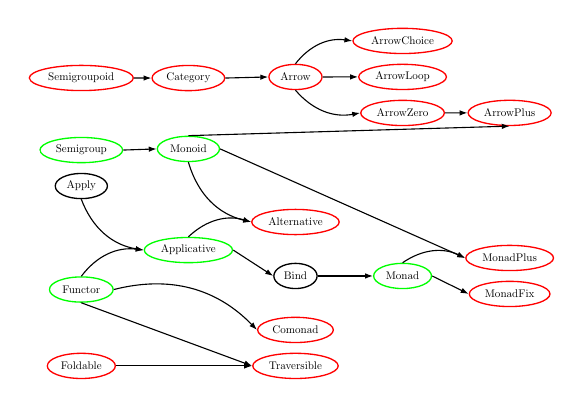
\begin{tikzpicture}
  [nodes={draw, ellipse, very thick, text=black, minimum size=0.8cm}, arrows={-Latex[length=1mm,width=0.7mm]}, level distance=3.4cm, grow'=right, sibling distance=0.3cm, scale=0.4]
  \tikzset{top/.style={color=red, text=black}}
  \tikzset{planned/.style={color=red, text=black}}
  \tikzset{half/.style={color=black, text=black}}
  \tikzset{done/.style={color=green, text=black}}
  \tikzset{root/.style={minimum size=0mm, minimum width=0mm, inner sep=0mm, outer sep=0mm, level distance=0mm}}
  \tikzset{level 1/.style={level distance=1.5cm}}

  \tikzset{edge from parent/.append style={white}}
  \Tree [.\node [root] (A) {};
  [.\node [planned] (SD) {Semigroupoid};
    [.\node [planned] (CA) {Category};
      [.\node [planned] (AR) {Arrow};
        [.\node [planned] (AC) {ArrowChoice};]
        [.\node [planned] (AL) {ArrowLoop};]
        [.\node [planned] (AZ) {ArrowZero};
          [.\node [planned] (AS) {ArrowPlus};]]]]]
  [.\node [done] (SG) {Semigroup};
    [.\node [done] (MD) {Monoid};]]
  [.\node [half] (AY) {Apply}; ]
  [.\node [done] (FU) {Functor};
    [.\node [done] (AP) {Applicative};
      [.\node [planned] (AT) {Alternative}; ]
      [.\node [half] (BI) {Bind};
        [.\node [done] (MO) {Monad};
          [.\node [planned] (MP) {MonadPlus}; ]
          [.\node [planned] (MF) {MonadFix};  ]]]]
    [.\node[root] (E1) {}; [.\node [planned] (CO) {Comonad}; ]]]
  [.\node [planned] (FO) {Foldable};
    [.\node[root] (E2) {}; [.\node [planned] (TR) {Traversible}; ]]]]

  \tikzset{edge from parent/.style={draw, very thick}}

  % Semigroupoid
  \draw (SD.east) -- (CA.west);
    % Category
    \draw (CA.east) -- (AR.west);
      % Arrow
      \draw (AR.north) to[bend left] (AC.west);
      \draw (AR.east) -- (AL.west);
      \draw (AR.south) to[bend right] (AZ.west);
        \draw (AZ.east) -- (AS.west);

  % Monoid
  \draw (SG.east) -- (MD.west);
  \draw (MD.north) -- (AS.south);
  \draw (MD.east) -- (MP.west);
  \draw (MD.south) to[bend right] (AT.west);

  % Apply
  \draw (AY.south) to[bend right] (AP.west);

  % Functor
  \draw (FU.north) to[bend left] (AP.west);
  \draw (FU.east) to[bend left] (CO.west);
  \draw (FU.south) -- (TR.west);
    % Applicative
    \draw (AP.north) to[bend left] (AT.west);
    \draw (AP.east) -- (BI.west);
      % Bind
      \draw (BI.east) -- (MO.west);
        % Monad
        \draw (MO.north) to[bend left] (MP.west);
        \draw (MO.east) -- (MF.west);

  % Foldable
  \draw (FO.east) -- (TR.west);
\end{tikzpicture}
\end{document}
